\documentclass[	DIV=calc,%
							paper=a4,%
							fontsize=11pt,%
							twocolumn]{scrartcl}	 					% KOMA-article class

\usepackage{lipsum}													% Package to create dummy text

\usepackage[english]{babel}										% English language/hyphenation
\usepackage[protrusion=true,expansion=true]{microtype}				% Better typography
\usepackage{amsmath,amsfonts,amsthm}					% Math packages
\usepackage[pdftex]{graphicx}									% Enable pdflatex
\usepackage[svgnames]{xcolor}									% Enabling colors by their 'svgnames'
\usepackage[hang, small,labelfont=bf,up,textfont=it,up]{caption}	% Custom captions under/above floats
\usepackage{epstopdf}												% Converts .eps to .pdf
\usepackage{subfig}													% Subfigures
\usepackage{booktabs}												% Nicer tables
\usepackage{fix-cm}	
\usepackage{color}
\usepackage{hyperref}
\usepackage{amsmath}
\usepackage{amssymb}
\usepackage{tikz}
\usepackage{tabularx}
\usepackage{amsmath}
\usepackage{layouts}
\usepackage{array}
\usepackage{tikz}
\usepackage{amssymb}
\usepackage{graphics}
\usepackage{lmodern}
\usepackage{epstopdf}
\usepackage[T1]{fontenc}
\usepackage[utf8]{inputenc}
\usepackage{authblk}
\usepackage{tabularx}
\usepackage{multirow}
\usepackage{bm}
\usepackage{here}
\usepackage{biblatex} 
\bibliography{report} 
\usepackage{enumerate}												% Custom fontsizes



%%% Custom sectioning (sectsty package)
\usepackage{sectsty}													% Custom sectioning (see below)
\allsectionsfont{%															% Change font of al section commands
	\usefont{OT1}{phv}{b}{n}%										% bch-b-n: CharterBT-Bold font
	}

\sectionfont{%																% Change font of \section command
	\usefont{OT1}{phv}{b}{n}%										% bch-b-n: CharterBT-Bold font
	}


\hypersetup{
  colorlinks,%
    citecolor=black,%
    filecolor=black,%
    linkcolor=black,%
    urlcolor=black
}

%%% Headers and footers
\usepackage{fancyhdr}												% Needed to define custom headers/footers
	\pagestyle{fancy}														% Enabling the custom headers/footers
\usepackage{lastpage}	

% Header (empty)
\lhead{}
\chead{}
\rhead{}
% Footer (you may change this to your own needs)
\lfoot{\footnotesize \texttt{NAO Localization} \textbullet ~University of Amsterdam}
\cfoot{}
\rfoot{\footnotesize page \thepage\ of \pageref{LastPage}}	% "Page 1 of 2"
\renewcommand{\headrulewidth}{0.0pt}
\renewcommand{\footrulewidth}{0.4pt}



%%% Creating an initial of the very first character of the content
\usepackage{lettrine}
\newcommand{\initial}[1]{%
     \lettrine[lines=3,lhang=0.3,nindent=0em]{
     				\color{DarkGoldenrod}
     				{\textsf{#1}}}{}}



%%% Title, author and date metadata
\usepackage{titling}															% For custom titles

\newcommand{\HorRule}{\color{DarkGoldenrod}%			% Creating a horizontal rule
									  	\rule{\linewidth}{1pt}%
										}

\pretitle{\vspace{-30pt} \begin{flushleft} \HorRule 
				\fontsize{50}{50} \usefont{OT1}{phv}{b}{n} \color{DarkRed} \selectfont 
				}
\title{NAO Localization}					% Title of your article goes here
\posttitle{\par\end{flushleft}\vskip 0.5em}

\preauthor{\begin{flushleft}
					\large \lineskip 0.5em \usefont{OT1}{phv}{b}{sl} \color{DarkRed}}
\author{Amogh Gudi, Georgios K. Methenitis, Nikolaas Steenbergen, Patrick de Kok\\}											% Author name goes here
\postauthor{\footnotesize \usefont{OT1}{phv}{m}{sl} \color{Black} 
					University of Amsterdam 								% Institution of author
					\par\end{flushleft}\HorRule}

\date{}																				% No date



%%% Begin document
\begin{document}
\maketitle
\thispagestyle{fancy} 			% Enabling the custom headers/footers for the first page 
% The first character should be within \initial{}
\initial{I}\textbf{n this Project we propose a basic code for the Robo soccer Standard league Platform for the Dutch national team. We focused on the problem of visual feature recognition and the localization of the robot in a tournament setup. This project contains a detailed description of our implementation together with a conclusion and a brief evaluation. Since this report only covers feature detection and Localization we give an outlook on what parts are to be implemented in addition to make the robots play soccer.}

\section{Feature Extraction}
Visual object recognition is a key ability for autonomous robotic agents especially in dynamic and partially observable environments. A reliable landmark detection process is really crucial for achieving self-localization, which can be easily considered as the stepping stone for having a functional robotic soccer team. In this section, we describe the whole procedure of processing input images from the NAO's camera, outputting features that are informative to be used by the core of our localization scheme.  Using a variety of image processing techniques, we successfully detect field landmarks. In general, we have to deal with noisy images, which not only contain the field region but also background noise and useless information which comes from above the horizon of the field view. Furthermore, we had to deal with lighting conditions which may vary significantly.
There also real-time constraints which had to be taken into consideration during our algorithmic implementation in order for the whole procedure to be able to execute in real time.

\begin{figure}[t!]
  \caption{HSV colorspace. \href{http://en.wikipedia.org/wiki/HSL_and_HSV}{( Image source )}}
  \label{hsv}
  \centering
    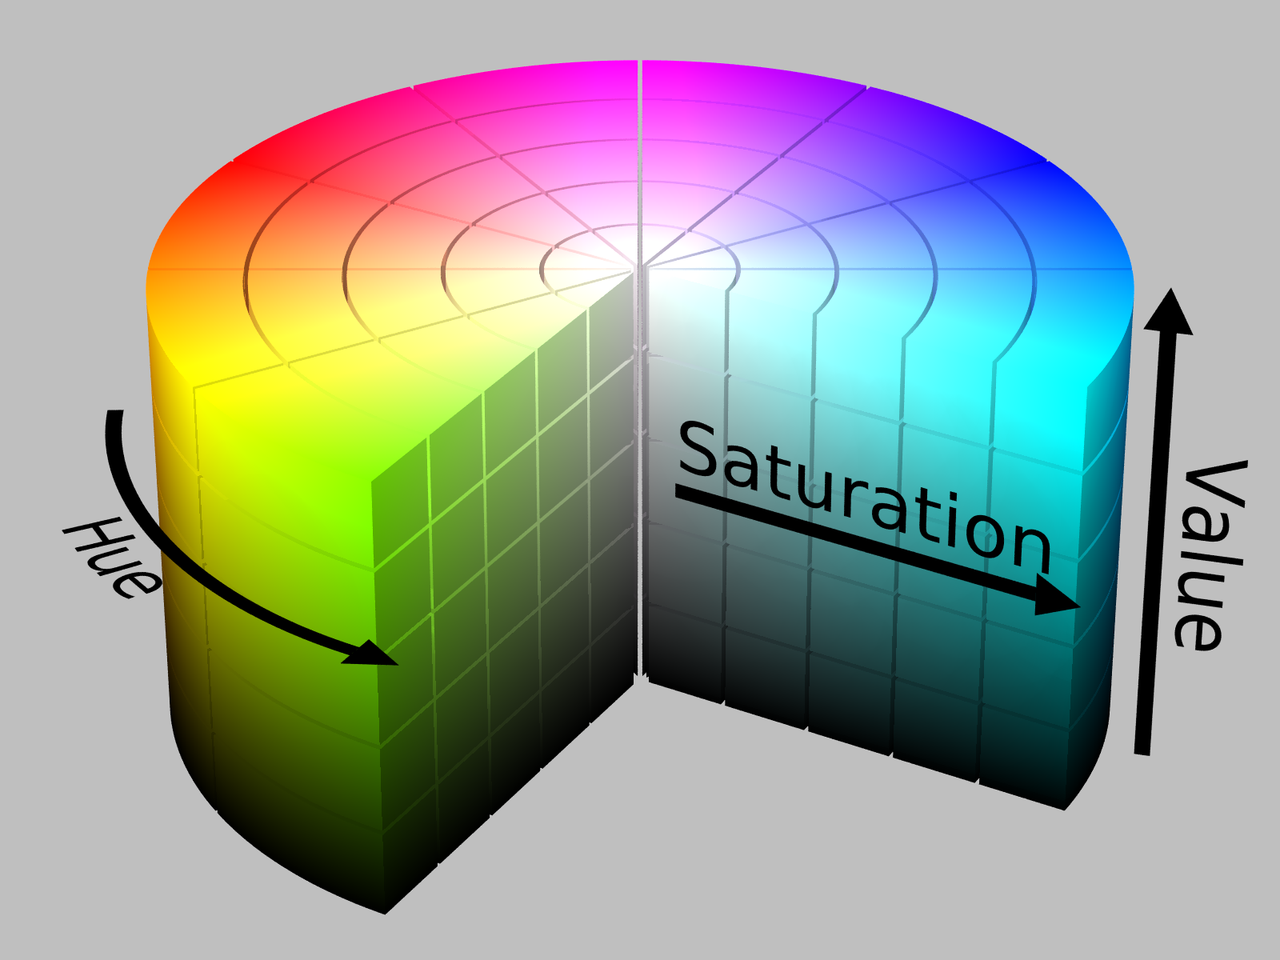
\includegraphics[width=0.3\textwidth]{figures/1280px-HSV_color_solid_cylinder_alpha_lowgamma.png}
\end{figure}

\subsection{Choosing colorspace}
The first challenge we came along was to choose the best colorspace representation in order to overcome the variations in lighting conditions. The dataset we had consisted from rgb images. Unfortunately, it was unfeasible to use the default rgb colorspace for most applications due to noise, shadows, etc. We also experimented with normalized rgb colorspace. Theoretically,  normalized rgb would have given us the pure chromaticity values of each object in our field of view, overcoming like this possible shadows and lighting conditions. In the contrary, normalized rgb did not help us achieving a light-invariant color representation, resulting into false positives in color segmentation. HSV was the solution to our problem. HSV is a cylindrical colorspace representation, which contains information about hue, saturation, and value. We found hue to be really informative in order to distinguish  easily between the colors. Hue define the pure chromaticity of the color and it is independent of the lighting conditions. In figure~\ref{hsv}, we illustrate this cylindrical color representation, we can see that the hue is represented by the angular dimension in the vertical axis of the cylinder. 


\subsection{Basic Pipeline}
Having described the first basic step of our approach, choosing the proper colorspace for our application, it is time to go deeper into the feature extraction procedure.
The first step in this procedure is the image input from the NAO's camera in HSV format. As we said before, images not only contain the important region of the field in which we are interested in, but also some background information which is useless in order to detect field features. This background usually extends above the field horizon and it may become really disturbing in the extraction process. This is the reason why background removal is the first step in our feature extraction scheme. Once we have removed, our input image contains information which has to be extracted. Field lines, goals, ball, and other NAO robots are the features located into the field. In this project, we only took into consideration lines, and the goals which are static landmarks, as ball, and other robots are moving and we cannot depend on them in order to self-localize. So, we use information from the HSV values to binarize the image, first in respect to the goals and then in respect to the lines. As we said in the introduction part of this paper, field is colored green, both goals are yellow, and lines are white. Next step of the feature extraction is the the goal detection, making use of the horizontal and vertical histograms of yellow values. Line detection is followed in order to find a good estimation about the lines detected in our field of view. Having these lines' estimations, we can detect feature on them, using geometric properties. Last step in this process' pipeline is to output all these detected features to the localization core process. We can now enumerate all steps in these pipeline, these are:
\begin{enumerate}
\item Input HSV image from camera
\item Background removal
\item Image binarization
\item Goal detection
\item Line detection
\item Line feature detection
\item Output features
\end{enumerate}

\section{Image format}
NAO's camera can output images in different colorspaces representations. The images from the dataset we had, were in RGB format, and they had QVGA resolution ($320 \times 240$). We wanted to keep a low resolution in order to keep the time complexity of our algorithm feasible for real-time execution. Patrick can add some things here as he experimented better with NAO's camera.































\end{document}